\documentclass[12pt, french]{report}

\usepackage{amsmath,amsthm,verbatim,amssymb,amsfonts,amscd, graphicx}
\usepackage[utf8]{inputenc}
\usepackage{babel}
\usepackage{enumitem}
\usepackage{amssymb}
\usepackage{amsmath}
\usepackage{mathrsfs}
\usepackage{graphicx}
\usepackage{yfonts}
\usepackage{amscd}
\usepackage[colorlinks=true, allcolors=blue]{hyperref}
\usepackage{cleveref}
\graphicspath{{images/}}
%%%%%%%%%%%%%%%%%%%%%%%%%%%%%%%%%%%%%%%%%%%%%%%%%%%%%%%%%%%%%%%%%%%%%%%%%%%%%%
\renewcommand{\contentsname}{Table des matières}
%\renewcommand{\refname}{Bibliographie}
\renewcommand{\baselinestretch}{1.05}

\theoremstyle{theoreme}
\newtheorem{theoreme}{Théorème}

%%%%%%%%%%%%%%%%%%%%%%%%%%%%%%%%%%%%%%%%%%%%%%%%%%%%%%%%%%%%%%%%%%%%%%%%%%%%%
\title{PRL}

\author{En-Hung Chao \\ Honghao Li}
\date{\today}
%%%%%%%%%%%%%%%%%%%%%%%%%%%%%%%%%%%%%%%%%%%%%%%%%%%%%%%%%%%%%%%%%%%%%%%%%%%%%%
%%%%%%%%%%%%%%%%%%%%%%%%%%%%%%%%%%%%%%%%%%%%%%%%%%%%%%%%%%%%%%%%%%%%%%%%%%%%%%
\begin{document}

\maketitle

\newpage
\tableofcontents

\newpage
\chapter{Introduction et motivation}
\addcontentsline{toc}{section}{Introduction}
Le calcium oxalate est un matériau riche dans la nature. Notamment, on peut le retrouver dans les calculs rénaux (communément appelés "pierres aux reins") qui sont formés par le calcium phosphalte, une plus grande structure qui contient les états hydratés du calcium oxalate. 
Pour étudier un tel matériau sans changer sa structure ou le détruire, on fait souvent des études spectroscopiques.
Cela consiste à étudier les propriétés optiques et diélectriques du matériau en analysant la réponse du matériau à une lumière incidente.
Typiquement, on peut déduire des spectroscopies de perte et d'absorption la fonction diélectrique (ou plutôt son inverse).
\\\\Dans le cadre du projet en laboratoire de l'École Polytechnique, nous avons choisi de faire le sujet proposé par M. Franceso Sottile du Laboratoire des Solides Iradiés de l'École Polytechnique (LSI), qui consiste à montrer des propriétés spectroscopiques du calcium oxalate par des calculs \textit{ab initio}. 
Il s'agit donc de bien comprendre la théorie de la fonctionnelle de la densité (\textit{Density Functional Theory} en anglais, DFT) et la théorie de la fonctionnelle dépendante du temps (\textit{Time-Depending Density Functional Theory} en anglais, TDDFT) et de les appliquer avec les codes existants.
La DFT et la TDDFT sont deux pilliers des calculs \textit{ab initio} qui donnent d'assez bonnes prédictions théoriques par rapport aux expériences réelles.

L'intérêt de notre travail serait de fournir une prédiction théorique et numérique sur les caractéristiques du calcium oxalate en basse énergie qui pourrait être consultée par des expérimentateurs intéressés par ce matériau. 
 

%%%%%%%%%%%%%%%%%%%%%%%%%%%%%%%%%%%%%%%%%%%%%%%%%%%%%%%%%%%%%%%%%%%%%%%%
\chapter{Études théoriques des systèmes à plusieurs corps}
\section{Le problème électronique}
Dans la physique des solides, on est ramené à étudier l'équation de Schrödinger d'un système à plusieurs corps ($N$ électrons et $M$ ions par exemple), ce qui consiste à résoudre une équation du type

\begin{equation}
\begin{split}
(\sum_{i=1}^N \frac{\textbf{p}_i^2}{2m_i} + \sum_{I=1}^M \frac{\textbf{P}_i^2}{2M_I}
+ \sum_{i<j}\frac{e^2}{| \textbf{r}_i - \textbf{r}_j |} - \sum_{i, I}\frac{Z_I e^2}{| \textbf{r}_i
- \textbf{R}_I |} + \sum_{I<J}\frac{Z_I Z_J e^2}{| \textbf{R}_i - \textbf{R}_j |} ) \Psi = E_{tot} \Psi
\end{split}
\end{equation}

où $(\textbf{r}, \textbf{p})$ et $(\textbf{R}, \textbf{P})$ sont respctivement la position et l'impulsion d'un éléctron et d'un proton, $E_{tot}$ est une certaine énergie propre du système qu'on voudra trouver et enfin, $\Psi = \Psi(\textbf{r}_1, \ldots, \textbf{r}_N,  \textbf{R}_1, \ldots \textbf{R}_M)$ est une fonction à $N+M $ variables.

Comme le système qu'on considère (les solides) comprend un nombre très élevé d'électrons et d'ions, cette équation ne peut pas être résolue analytiquement, voire numériquement. On doit appliquer certaines approximations au système afin de réduire la complexité du calcul. La première approximation qu'on peut prendre, celle la plus intuitive, est celle de Born-Oppenheimer.~\cite{Bor27}
En tenant compte du rapport de masse entre les électrons et les ions et en supposant que les ions sont quasiment figés par rapport aux électrons (ayant une longueur d'onde de De Broglie plus élevée), on peut réécrire l'hamiltonien du système d'électrons comme

$$
H = \underbrace{\sum_{i=1}^N \frac{\textbf{p}_i^2}{2m_i}}_{T}
+ \underbrace{\sum_{i<j}\frac{e^2}{| \textbf{r}_i - \textbf{r}_j |}}_{V}
- \sum_i V_{ext}(\textbf{r}_i)
$$
où $T$ est l'énergie cinétique des électrons, $V$ leur énergie potentielle d'interaction et $V_{ext}$ l'énergie potentielle dûe à l'extérieur due aux ions fixés.
Notre problème devient

$$
H \Psi_e(\textbf{r}_1, \ldots \textbf{r}_N) = E_{tot} \Psi_e(\textbf{r}_1, \ldots \textbf{r}_N)
$$

Or, le problème n'est toujours pas simple car la fonction d'onde $\Psi_e$ que l'on cherche est une fonction à plusieurs variables. 

\subsection{Théorie de la fonctionnelle de la densité (\textit{DFT} en anglais)}
\subsection{La méthode de Kohn et Sham}
\label{subsec-KS}
Si les électrons étaient non-interagissant entre eux, on pourrait écrire l'hamiltonien comme une somme de plusieurs hamiltoniens d'un seul électron, \textit{i.e.},

$$
H = \sum_i H_i^{(1e)} = \sum_i ((-\frac{\hbar^2}{2m}\nabla_i^2 + V_{eff}(\textbf{r}_i))
$$

Le théorème développé par Hohenberg et Kohn~\cite{Hoh64} nous donne la possibilité d'approximer la vraie solution en passant par un système auxiliaire d'électrons non-interagissants.

\begin{theoreme}[Hohnenberg-Kohn]
  La valeur d'espérance d'un observable dans l'état fondamental est l'unique fonctionnelle de la densité d'électron.
\end{theoreme}

La preuve de ce théorème peut être trouvée dans~\cite{Hoh64}.
Ce résultat implique que la valeur d'espérance de l'hamiltonien à l'état fondament total, donc l'énergie fondamentale du système, est une fonctionnel de la densité d'électrons $n(\textbf{r}) = \sum_i \int |\Psi_e(\textbf{r}_1, \ldots \textbf{r}_N) |^2 \delta (\textbf{r} - \textbf{r}_i) \prod_{j=1}^N d\textbf{r}_j$.

Grâce à ce théorème, la résolution d'un système à plusieurs corps devient la recherche d'une fonctionnelle réelle dépendant uniquement d'une variable spatiale. La résolution va être plus simple à implémenter par rapport à la recherche de la fonction d'onde à plusieurs variable $\Psi (\textbf{r}_1, \ldots, \textbf{r}_N)$ du problème initial.

L'article~\cite{Koh65} de Kohn et Sham fournit un autre pillier de la DFT. La méthode de Kohn et Sham consiste à poser un système auxiliaire d'hamiltonien $H' = T' + V'_{tot}$, qui a le même densité d'électrons que notre vrai système $H = T + V + V_{ext}$. Ce système auxiliaire étant non-interagissant, on peut donc prendre pour la densité $n(\textbf{r}) = n'(\textbf{r}) = \sum_i |\phi_i(\textbf{r})|^2$ ,avec la fonction d'onde totale du système s'exprime par $\Psi(\textbf{r}_1 \ldots \textbf{r}_N) = \prod_i \phi_i(\textbf{r})$. On peut donc considérer le système d'équation suivant

$$
(-\frac{1}{2}\nabla_i^2 + V_{tot}[n](\textbf{r}))\phi_i(\textbf{r}) = \epsilon_i \phi_i (\textbf{r})
$$

avec
\begin{equation}\label{Vtot}
V_{tot}(\textbf{r}) = V_{ext}(\textbf{r}) + \int d\textbf{r}' \frac{n(\textbf{r}')}{|\textbf{r} - \textbf{r'}|} + V_{xc}([n], \textbf{r})
\end{equation}

pour chacun des électrons $i$. Le problème devient un problème simple de $N$ équations à une variable (en $\phi_i(\textbf{r})$) séparées. On pourra ensuite faire une résolution auto-consistente en réinjectant $n = \sum_i |\phi_i^{(p)}(\textbf{r})|^2 $ après chaque itération $p$. (L'auto-consistence de cette méthode n'a toujours pas été prouvée.) Une fois minisé l'énergie totale du système auxiliaire $\langle \Psi_e | H' | \Psi_e \rangle $, on obtiendra la densité exacte $n(\textbf{r})$ du vrai système, ce qui nous permettra de trouver l'énergie de l'état fondamental.

Cependant, il y a une approximation à faire pour le terme du potentiel d'échange-corrélation $V_{xc}(\textbf{r}) = \frac{\delta E_{xc}}{\delta n(\textbf{r})}$, où

\begin{equation}
\label{eqn-exc}
  E_{xc} = T[n] + V[n] - \frac{1}{2}\int d\textbf{r}
  \int d\textbf{r}' v(\textbf{r}, \textbf{r}') n(\textbf{r}) n(\textbf{r'}) - T'[n]
\end{equation}

La DFT est aujourd'hui la méthode la plus utilisée pour étudier les propriétés de l'état fondamental d'un système (module d'élasticité, stabilité de la structure, vibrations phononiques, etc)~\cite{Mar04}

%17/02/2017%%%%%%%%%%%%%%%%%%%%%%%%%%%%%%%%%%%%%%%%%%%%%%%
\section{Théorie de la fonctionelle de la densité dépendante du temps}\label{sec-TDDFT}
Dans les études de spectroscopie, nous étudions les comportements des matériaux sous exicitation. La constante diélectrique et son inverse sont par exemple des grandeurs physiques que l'on regarde souvent dans les expériences (déduites à partir de l'absorption et de la réflexion des lumières, cf.~\cite{Sot03} Chap. 1). Par conséquent, la simple étude de l'état fondamental ne suffit pas, il nous faut de plus des études sur les états excités.

La méthode que nous allons présenter dans ce rapport, la théorie de la fonctionelle de densité dépendante du temps (\textit{Time-Depending Density Functional Theory}), est utilisée dans le code à l'aide duquel on fait des simulations numériques \textit{ab initio}. 

\subsection{TDDFT}
La TDDFT est une extension de la DFT. Grâce au théorème de Runge et Gross~\cite{Run84}, il est possible d'affirmer que la valeur moyenne de toute observable $\hat{O}$ dépendante du temps est l'unique fonctionelle de la densité d'électrons dépendants du temps. Ceci s'exprime mathématiquement par

$$
\langle \Psi (\textbf{r}_1, \ldots, \textbf{r}_N, t) | \hat{O} | \Psi (\textbf{r}_1, \ldots, \textbf{r}_N, t) \rangle = \hat{O}[n(t)]
$$

Ici, la densité dépendante du temps est la variable fondamentale exactement comme pour le cas statique. La dépendence du temps de la densité provient du fait que le système est soumis à un champ extérieur dépendant du temps. La TDDFT est valable pour n'importe quel type de potentiel extérieur. Ici, nous nous intéressons en particulier aux cas où le potentiel extérieur est "petit", ce qui nous permet de rentrer dans le cadre de la \textbf{réponse linéaire} (cf. Annexe~\ref{TRL}). En fait, comme expliqué dans l'introduction, 

%TODO vérifier si on l'a bien mis dans l'intro

la fonction diélectrique du système $\epsilon^{-1}$ est lié aux propriétés optiques et diélectriques d'un matériau.

Nous allons étudier le comportement de la fonction diélectrique du système en présence d'une excitation extérieure en régime linéaire. La relation entre le potentiel d'perturbation extérieure et le potentiel total à l'intérieur du système est donnée par (dans l'espace réciproque de transformation de Fourier temporelle)

\begin{equation}\label{VtotVext}
V_{tot}(\textbf{r}, \omega) = \int d\textbf{r}' \epsilon^{-1}(\omega) V_{ext}(\textbf{r}', \omega)
\end{equation}

On notera $\chi^0$ et $\chi$ les fonctions de réponse linéaire pour $V_{tot}$ et $V_{ext}$ respectivement (cf. Annexe~\ref{TRL} pour la définition de ces fonctions). On a les relations entre la fonctionelle de densité $n$ et ces deux potentiels

$$
n(\textbf{r}, t) = \int d\textbf{r}' dt' \chi^0(\textbf{r}, \textbf{r'}, t-t') V_{tot}(\textbf{r}', t) = \int d\textbf{r}' dt' \chi(\textbf{r}, \textbf{r'}, t-t') V_{ext}(\textbf{r}', t)
$$

%TODO l'expression de chi ??

Enfin, la relation entre $\chi^0$ et $\chi$ peut être donnée de façon plus explicite en utilisant la méthode variationnelle

\begin{equation}
  \label{eqn-chi0chi}
  \chi = \frac{\delta n}{\delta V_{ext}}
       = \frac{\delta n}{\delta V_{tot}} \frac{\delta V_{tot}}{\delta n}
       = \chi^0 ( 1 + (v+f_{xc})\chi)
\end{equation}

où nous avons utilisé l'expression de $V_{tot}$ de l'équation~\ref{Vtot}, $v = \frac{\delta V_H}{\delta n}$ pour la variation du deuxième terme dans l'expression de $V_{tot}$ (potentiel de Hatree) et $f_{xc} = \frac{\delta V_{xc}}{\delta n}$. À noter que les convolutions sont remplacées par les multiplications ici pour la raison de simplicité d'écriture.


\subsection{Coefficient diélectrique et fonction de perte}
\label{subsec-eels}
Dans une vraie expérience de spectroscopie, on mesure l'absorption (Abs) et les spectres de perte d'énergie d'électron (\textit{Electron Energy Loss Spectra} en anglais, EELS). Ces deux grandeurs physiques sont liées à la fonction diélectrique (~\cite{Sot03}, Sect. 1.5)

$$
Abs = \mathfrak{I}(\epsilon) \quad EELS = -\mathfrak{I}(\epsilon^{-1})
$$

Abs nous indique les fréquences de la lumière que le système peut absorber. EELS nous donne une idée sur les fréquences et les moments que le système peut échanger avec un projectile extérieur (photon ou électron). Les deux nous donnent donc les caractéristiques intrinsèques du système. Pour ces observables, la fonction diélectrique $\epsilon$ est liée à la fonction de la réponse linéaire par~\cite{Sot03}

\begin{equation}\label{epsilon}
  \epsilon^{-1} = 1+ v\chi
\end{equation}

L'intérêt principal de notre travail est donc de prédire le comportement de $\epsilon$ du matériau choisi quand des photos de certaines énergies y sont envoyés.

Dans la suite de ce rapport, nous allons présenter les aspects numériques de notre projet, dont les codes qui exploitent les relations que l'on vient d'établir.

%%%%%%%%%%%%%%%%%%%%%%%%%%%%%%%%%%%%%%%%%%%%%%%%%%%%%%%%%%
\chapter{Simulations numériques}
\label{chap-simulation}
Nos travaux ont été réalisés en deux temps.
Nous commençons par étudier l'état fondamental du calcium oxalate à l'aide du logiciel \textit{Abinit}~\cite{Abinit}.
Après, nous utilisons le code \textit{DP}~\cite{DP} pour étudier les états excités
en servant des résultats obtenus dans l'étape précédente.

Les fonctionnements des outils, aussi bien que les approximations impliquées,
seront présentées au cours de ce chapitre, suivies par l'explicitation du schéma de la simulation.

\section{Abinit}
\label{sec-abinit}
Abinit est un logiciel qui implémente numériquement la théorie de la fonctionnelle de la densité.
Il nous permet de faire des calculs ab initio pour obtenir la densité électronique,
et ainsi l'énergie fondamentale du système.
Plus précisément, Abinit effectue la résolution auto-consistente pour le système d'équations de Kohn et Sham à l'aide une base d'ondes planes.
A chaque itération, le point minimum d'énergie est calculé par la méthode du gradient conjugué,
et l'approximation du pseudo-potentiel est introduite pour éliminer dans le systéme d'équations les électrons de cœur,
ce qui réduit considérablement la complexité du probleme.

Avant de démarer le calcul,
plusieurs paramètres doivent être spécifiés pour la résolution numérique.
Du côté physique, le système étudié étant cristallin,
il faut d'abord définir la maille élémentaire.
Du côté technique, il faut préciser les méthodes utilisées et des valuers critiques qui gouvernent le comportement du calcul.
Dans la suite, nous proposons d'abord quelques approximations importantes. Ensuite,
Nous présentons les paramètres principaux qui nous servent dans notre études.
Une liste complète des paramètres utilisés se trouve dans l'annexe.

\subsection{Espace réciproque}
\label{subsec-reciprocal}
La partie éssentielle du calcul avec Abinit consiste à résoudre le système d'équations de Kohn et Sham,
dont la quantité clée est la densité d'électrons $n(\V{r})$.
Or les système étudiés sont souvent des matériaux cristallins,
auxquels on applique la condition périodique aux limites.
D'après le théorème de Bloch, les états propres, et ainsi les fonctions d'ondes correspondantes,
sont caractérisés par deux nombres quantiques:
le vecteur d'onde $\vb{k}$ dans la première zone de Brillouin, et l'indice de bande $n$.
La densité de charge s'exprime donc par
\begin{equation}
  \label{eqn-den}
  n(\vb{r}) = \sum_{n, \vb{k}}^\V{occ}\abs{\phi_{n, \vb{k}}(\vb{r})}^2,
\end{equation}
avec la somme sur tous les états occupés.
A la limite des cristaux idéals infinis, la taille de grille dans l'espace réciproque tend vers zéro,
alors l'\cref{eqn-den} devient
\begin{equation*}
  n(\vb{r}) = \sum_n^\V{occ}\int_{\V{ZB}}\dd[3]{\vb{k}}\abs{\phi_{n, \vb{k}}(\vb{r})}^2
\end{equation*}
où ZB signifie la première zone de Brillouin. Ensuite, à l'approximation numérique,
l'intégral sur $\vb{k}$ doit être discrétisée en somme sur $N_{\vb{k}}$ point $\vb{k}$ pondérés:
\begin{equation*}
  n(\vb{r}) = \sum_n^\V{occ}\sum_{i=1}^{N_{\vb{k}}}\abs{\phi_{n, \vb{k}}(\vb{r})}^2.
\end{equation*}
Le temps de calcul étant proportionnel à $N_{\vb{k}}$,
il est donc nécessaire de choisir les points $\vb{k}$ afin de reproduire le résultat
de l'intégral avec la moindre erreur et le moindre nombre de point $\vb{k}$.
Une méthode très utilisée est basée sur les travaux de Monkhorst et Pack~\cite{Monkhorst1976}.
L'idée est d'abord de prendre une grille homogène de points $\vb{k}$ dans la zone de Brillouin
qui respecte les symétries du réseau cristallin,
et ensuite d'augmenter la densité du grillage (et ainsi celle du nombre total de point $\vb{k}$)
jusqu'à la convergence, par example, de l'énergie totale du système.

\subsection{Base d'ondes planes}
\label{subsec-planewave}
La transformation de Fourier est très souvent lié avec la périodicité du système étudié.
Il est alors naturel de choisir, dans le contexte de l'approximation numérique,
la base d'ondes planes pour approximer les fonctions d'onde des états propres $\phi_i = \phi_{n,\vb{k}_i}$.
La théorème de Bloch nous donne:
\begin{equation*}
  \phi_{n,\vb{k}_i}
  = \frac{1}{\sqrt{\Omega_{\V{maille}}}}e^{i\vb{k}_i\vdot\vb{r}}\sum_{\vb{G}} c_{n,\vb{k}_i}(\vb{G})e^{i\vb{G}\vdot\vb{r}}
  = e^{i\vb{k}_i\vdot\vb{r}} u_{n,\vb{k}_i}(\vb{r})
\end{equation*}
où $u_{n,\vb{k}_i}(\vb{r})$ a la même périodicité que la structure cristalline
et $\vb{G}$ est un vecteur de réseau dans l'espace réciproque.
La base d'ondes planes nous donne les avantages suivants:
\begin{itemize}
  \item[-] La simplification des calculs de dérivé et d'intégral,
    qui apparaissent dans le calcul des éléments de l'hamiltonien.
  \item[-] Elle nous permet la méthode FFT pour des transformations rapides entre l'espace réel et l'espace réciproque.
  \item[-] L'ensemble d'ondes planes est complèt et orthonormal.
  \item[-] La base est de dimension infinie, mais le coupage de la dimension peut être réalisé facilement
    par la définition d'un seuil d'énergie $E_{\V{cut}}$:
    \begin{equation}
      \frac{1}{2}|\vb{k}+G|^2 \leq E_{\V{cut}}
    \end{equation}
    qui relie le nombre d'ondes planes dans la base et $E_{\V{cut}}$ par
    \begin{equation}
      N_{\V{op}}\propto E_{\V{cut}}^{\frac{3}{2}}.
    \end{equation}
    Une étude de la convergence de l'énergie totale du système par rapport à ce seuil de coupage est alors nécessaire.
\end{itemize}

\subsection{Pseudo-potentiel}
\label{subsec-pseudo}
Le nombre total d'électrons du système étudié étant souvent énorme,
beaucoup d'entre eux se trouvent proche des ions.
Ensemble avec les ions, ces électrons de cœur contribuent seulement de façon paramétrique
àux caractéristiques chimiques du système.
Cependant, ils apparaissent dans les termes d'interaction entre électrons avec les électrons de conduction.
I'idée essentielle du pseudo-potentiel est donc de simuler l'effet des ions et des électrons de cœur
sur les électrons de valence par un potentiel effectif qui donne aux électrons de valence
les même values propres et caractéristiques de ``scattering'' que le système réel.
Un premier avantage de l'introduction de pseudo-potentiel est la réduction du nombre d'électrons dans l'hamiltonien.
Un autre avantage moin évident mais aussi important est la réduction du seuil d'énergie des ondes planes introduit dans la \cref{subsec-planewave},
c'est-à-dire l'augmentation de l'efficacité du calcul, car les pseudo-potentiels sont beaucoup moin abrupts
que les vrais potentiels d'atome qui diverge près de l'origine,
ce qui signifie un moindre nombre de modes nécessaire dans la transformation de Fourier.
Dans notre études, nous utilisons les pseudo-potentiels fournis par le site d'Abinit pour toute les
quatre espèces d'atome (Ca, C, O, H)~\cite{Pseudo}.

\subsection{Potentiel d'échange-corrélation}
\label{subsec-xc}
Une dernière approximation importante engagé dans l'implémentation numérique
de la méthode de Kohn et Sham est celle sur l'énergie d'échange-corrélation (cf. \cref{eqn-exc}).
Par définition, $E_{\V{xc}}[n]$ contient tous les éffets au delà du formalisme de Hartree.
L'\cref{eqn-exc} étant exacte, l'expression explicite de $E_{\V{xc}}[n]$ est toujours inconnue,
d'où provient l'approximation.

Il existe beaucoup de méthodes d'approximation,
dont certaines sont présentées dans~\cite{Sottile2003}.
Dans nos études, l'approximation utilisée est celle de la densité locale (\textit{Local Density Approximation}, LDA),
l'idée principale de laquelle consiste à remplaçer la dépendance fonctionnelle de $E_{\V{xc}}[n]$
sur la distribution de la densité par celle sur la valeur locale de la densité.
Autrement dit, on suppose que l'énergie d'échange-corrélation du système à un point $\vb{r}$
est égale à celle d'un système homogène qui a la même valeur de la densité d'électrons au point $\vb{r}$.
Par conséquent, $E_{\V{xc}}[n]$ peut s'écrire sous la forme
\begin{equation}
  \label{eqn-exc-lda}
  E_{\V{xc}}^{\V{LDA}}[n] = \int n(\vb{r})\epsilon_{\V{xc}}(n(\vb{r})) \dd{\vb{r}}.
\end{equation}
L'intéret de cette forme est que $\epsilon_{\V{xc}}$ dans l'\cref{eqn-exc-lda} peut être obtenu avec
une précision suffisante par la méthode de Monte-Carlo quantique~\cite{ceperley1980}.
On attend un calcul exact par cette méthode pour un système homogène,
et ainsi de bonne approximation pour les systèmes dont la variation spatiale de la densité d'électrons est faible.
En fait, la portée de la méthode LDA va bien au delà de cette échelle,
et elle s'applique bien dans le domaine du semi-conducteur.
Une démonstration de cet applicabilité est présentée dans~\cite{Sottile2003}.

\section{DP}
DP est un code qui permet de calculer le coefficient diélectrique
en fonction de la fréquence et du moment transféré.
Dans le cas d'une simulation d'absorption,
$\vb{q}=0 \text{et} \omega = \text{la fréquence du photon absorbé}$.
Alors que dans le cas d'une simulation de perte d'énergie,
$\vb{q}= \text{le moment transféré et} \omega = \text{la perte d'énergie du projectile}$.
Il implémente la théorie détaillée dans la \cref{sec-TDDFT}.

\subsection{Noyau d'échange-corrélation}
Comme dans la méthode de Kohn et Sham (cf. \cref{subsec-KS}),
un terme dit le noyau d'échange-corrélation est introduit (cf. \cref{eqn-chi0chi})
pour tenir en compte tous les effets dynamiques d'échange et de corrélation
exercés par le potentiel externe.
À nouveau, ce terme doit être approximé car son expression explicite est inconnue.
Les méthodes d'approximation que nous utilisons dans le cadre de ce projet est
la \textit{Random Phase Approximation} (RPA) et
la \textit{Adiabatic Local Density Approximation} (ALDA).
La première approche, qui est aussi la plus simplifiée, prend un noyau nulle et
néglige donc les effets mentionnés ci-dessus.
La seconde approche, qui est largement utilisée,
prend le noyau comme la dérivée fonctionnelle du potentiel d'échange-corrélation
définie dans la \cref{subsec-KS}:
\begin{equation*}
  f_{\V{xc}}^{\V{ALDA}}(\vb{r}, \vb{r}')
  = \delta(\vb{r}, \vb{r}')\pdv{V_{\V{xc}}^{\V{LDA}}(n(\vb{r}), \vb{r})}{n(\vb{r})}.
\end{equation*}


\chapter{Resultats}


\label{Chap-Res}

\paragraph{Structure moléculaire du calcium oxalate}
%TODO add reference
La cellule élémentaire de calcium oxalate ($Ca C_2 O_4$) contient 28 atomes. Il est de structure monoclique et de groupe de symétrie $P2/m$ ($#$10) (cf. figure \ref{BrillouinZone})
%TODO add bilbao

\begin{figure}[!h]\label{BrillouinZone}
    \centering
    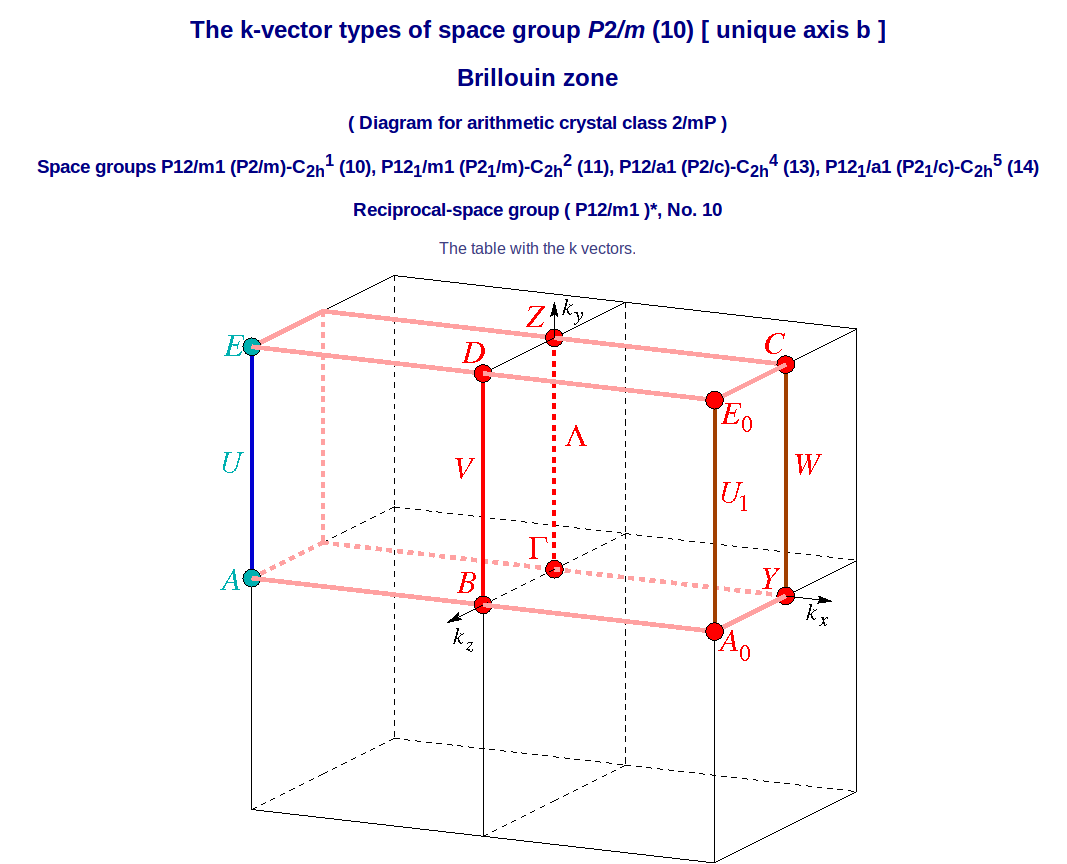
\includegraphics[width=8cm]{BrillouinZone}
    \caption{aldarpa}
\end{figure}
%%%%%%%%%%%%%%%%%%%%%%%%%%%%%%%%%%%%%%%%%
\paragraph{Ecut}
Pour commencer, on étudie la convergence du calcul de l'état fondamental de calcium oxalate. On fait varier le seuil d'énergie $E_{cut}$ entre 20 et 100 Hatree. 
On constate que pour tous ces seuils d'énergies, on obtient bien une convergence au bout de 15 itérations. La relation entre l'énergie totale du système à la convergence en fonction de l'énergie de seuil est tracée dans la figure \ref{Ecut}. 
À partir de $E_{cut} = 40$ Hatree, l'énergie totale du système est bien minimisée. On choisit donc cette énergie de seuil pour la suite du calcul de l'état fondamental. 

\begin{figure}[!h]\label{Ecut}
    \centering
    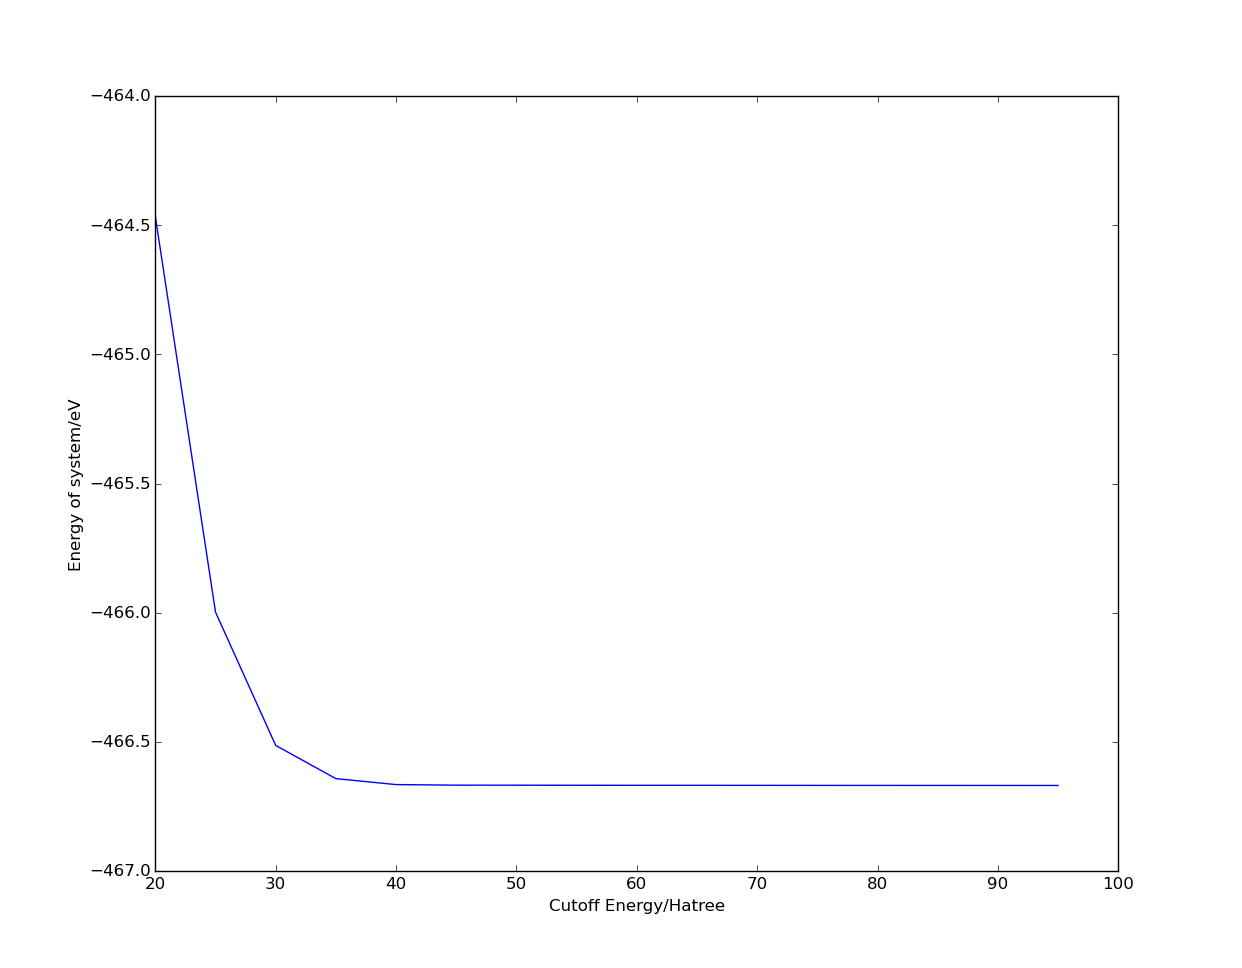
\includegraphics[width=8cm]{E_cut}
    \caption{Ecut}
\end{figure}

%TODO ajouter la structure de bandes

Dans un premier temps, avant de passer à l'état exicité, on peut construire sa structure de bandes à l'aide du calcul d'Abinit (cf. figure \ref{BrillouinZone}). 
Il est à remarquer que la structure de bande des états exicités seront différents que celle de l'état fondamental. 
Cependant, on pourrait avoir des idées sur celle des états excités. 
Notamment, le gap de la structure de bande montre que le calcium oxalate n'est pas un conducteur. 
Par ailleurs, comme le gap n'est pas direct, on peut donc observer des lumières émises dans des directions non parallèles à la lumière incidente. 

%%%%%%%%%%%%%%%%%%%%%%%%%%%%%%%%%%%%%%%%%%%%%%

\paragraph{rpa kpt compare} 
On crée des fichiers décrivant la fonction d'onde de l'état fondamental avec des échantillonnages de la première zone de Brillouin différents, où dans la première zone de Brouillin, il y a respectivement 16, 120 et 480 points-k. 
La motivation est de pouvoir avoir un échantillonnage assez fin pour obtenir tous les états d'excitation possibles sans avoir trop de points-k, ce qui demandera un temps de calcul considérable.
%TODO verifier si les parametres sont bien mentionnes auparavant
Pour connaître le meilleur échantillonnage à utiliser à notre disposition, on fait d'abord les calculs en prenant RPA (ramdom phase approximation) comme méthode d'approximation du terme d'échange et de corrélation.
Les résultats sont montrés dans la figure \ref{kptCompare}. 
On peut remarquer que les résultats pour 120 points-k et pour 480 points-k sont quasiment identiques en basses énergies (< 20 eV).
On choisit donc l'échantillonnage de 120 points-k pour continuer.

\begin{figure}[!h]\label{kptCompare}
    \centering
    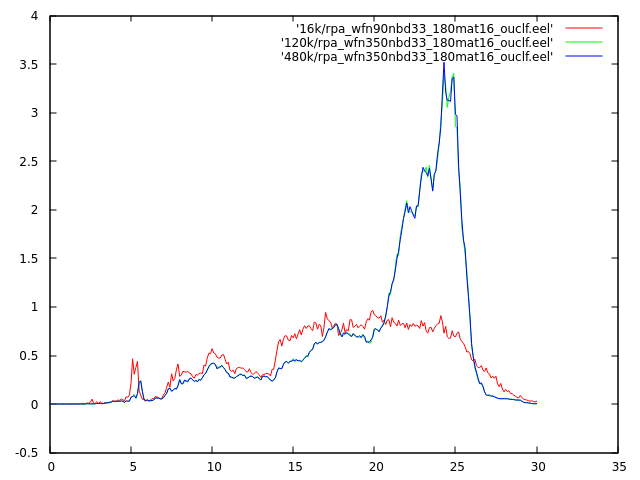
\includegraphics[width=8cm]{rpa_kpt_compare}
    \caption{rpa}
\end{figure}

%%%%%%%%%%%%%%%%%%%%%%%%%%%%%%%%%%%%%%%%%%%%%%%%%%%%%%%%%%%%%%%
La méthode d'approximation RPA prend moins de temps pour le calcul mais pourrait perdre la précision. Il est donc judicieux de comparer les résultats obtenus en appliquant RPA avec ceux obtenus en appliquant ALDA (adiabatic local density approximation).
Les deux approximations nous donnent des résultats assez proches en basses énergies.
Dans le cadre de ce projet, on se contente d'étudier les caractéristiques de calcium oxalate en basses énergie en raison du délai.
Il est donc tout à fait pertinent de faire notre calcul en RPA pour gagner en temps de calcul.
\paragraph{alda vs rpa}\label{aldaRPA}
\begin{figure}[!h]
    \centering
    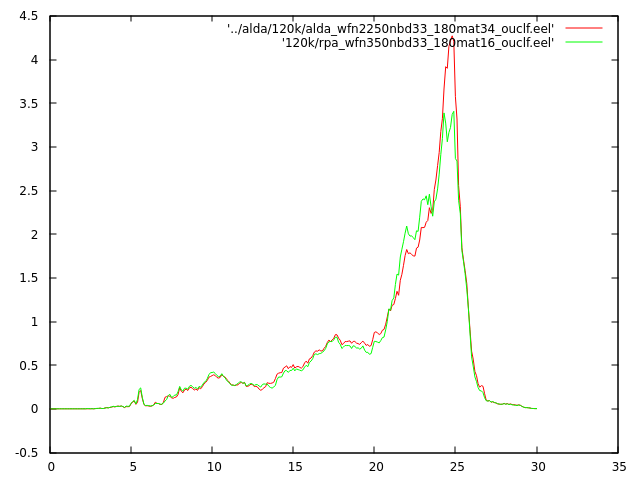
\includegraphics[width=8cm]{alda_vs_rpa}
    \caption{alda}
\end{figure}
%%%%%%%%%%%%%%%%%%%%%%%%%%%%%%%%%%%%%%%%%%%%%%%%%%%%%%%555555555%%%%%


\begin{figure}[!h]\label{CVwfnshRPA}
    \centering
    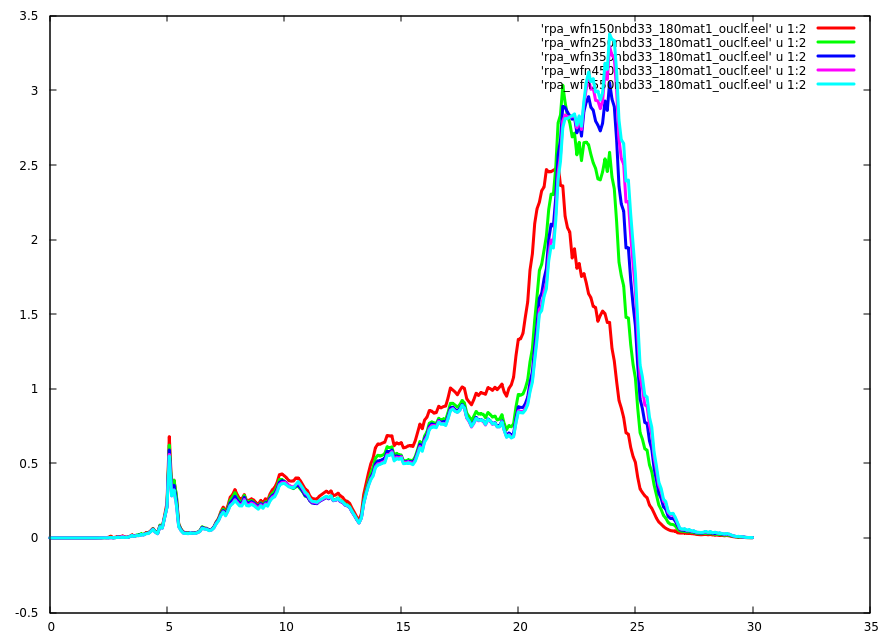
\includegraphics[width=8cm]{cv_wfnsh_rpa}
    \caption{alda}
\end{figure}

\paragraph{q6}
\begin{figure}[!h]
    \centering
    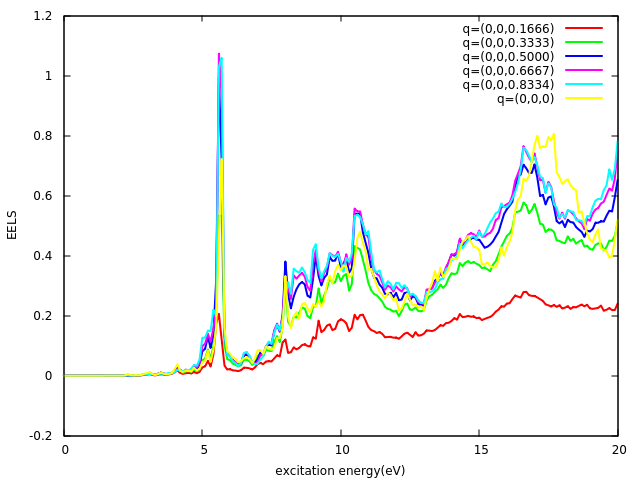
\includegraphics[width=8cm]{q6}
    \caption{}
\end{figure}


\paragraph{q8}
\begin{figure}[!h]
    \centering
    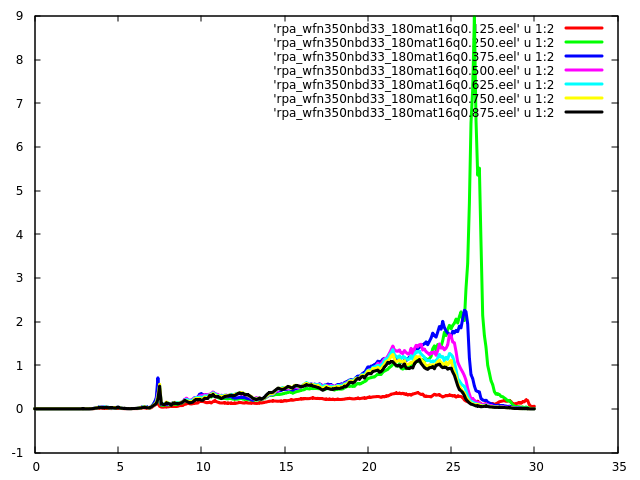
\includegraphics[width=8cm]{q8}
    \caption{rp}
\end{figure}


\paragraph{q10}
\begin{figure}[!h]
    \centering
    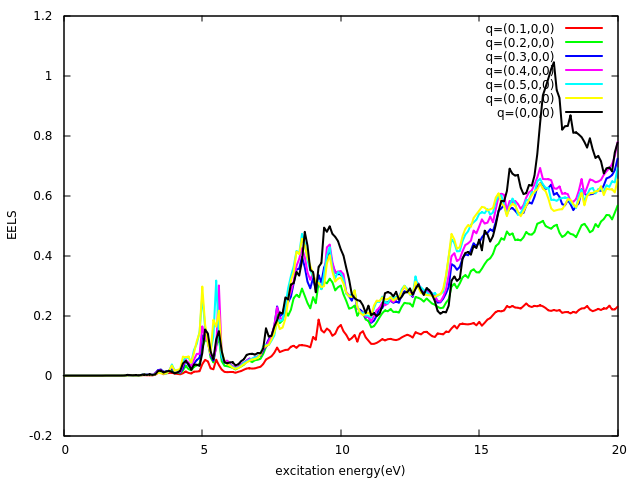
\includegraphics[width=8cm]{q10}
    \caption{rpa}
\end{figure}

\appendix
\chapter{Théorie de la réponse linéaire}\label{TRL}
Soit $n$ un observable. On suppose que $n$ varie en fonction de la perturbation $V$ de par

$$
n(\textbf{r}, t) = \int dt d\textbf{r'}  \chi (\textbf{r}, \textbf{r'}, t-t') V(\textbf{r'}, t')
$$

La fonction $\chi$ s'appelle la \textit{foncition de réponse linéaire}. Dans le cas où le hamiltonien de perturbation dépend aussi de $n$ par la relation suivante

$$
H = \int n(\textbf{r}, t) V(\textbf{r}, t) d\textbf{r}
$$

la fonction de réponse linéaire $\chi$ est donnée par la formule de Kubo\cite{Ton12}

\begin{equation}\label{kubo}
  \chi (\textbf{r}, \textbf{r}', t-t') = -i \langle N | [n(\textbf{r}, t), n(\textbf{r}', t)] |N \rangle \Theta(t-t')
\end{equation}

où $|N \rangle $ désigne l'état dans lequel on mesure l'observable $n$.

Nous supposons que la structure de bande obtenue à partir de l'état fondamental nous fournisse une base complète. Nous partons de $|N \rangle$ l'état fondamental constitué de $N$ électrons dans~\ref{kubo}. Notons $| j_N \rangle $ le j-ième état excité de notre système à $N$ électrons. En faisant la transformation de Fourier temporelle, la fonction de réponse linéaire s'écrit dans ce cas

\begin{equation}
\chi (\textbf{r}, \textbf{r}', \omega) = \sum_j \frac{f_j(\textbf{r}) f_j^*(\textbf{r}') }{\omega - \Omega_j + i \eta} + \frac{f_j(\textbf{r}') f_j^*(\textbf{r}) }{\omega + \Omega_j + i \eta}
\end{equation}

où $f_j = \langle N | n(\textbf{r}, 0) | j_N \rangle$, $\Omega_j = (E_0 - E_j)$ la différence d'énergie entre l'état $j$ et l'état fondamental et enfin $\eta$ le terme de lissage (\textit{broadening}) qui est à tendre vers 0 pour le calcul théorique.

Notons $n$ la fonciton de densité. C'est un observable obtenu à partir de la relation suivante

$$
n = \psi^\dagger \psi
$$

où $\psi$ est l'opérateur d'annihilation et $\psi^\dagger$ l'opérateur de création de l'état que l'on considère (en analogie avec les oscillateurs harmoniques).

On peut développer $\psi$ (et donc $\psi^\dagger$) dans la base des opérateurs de création
pour un seul électron.

$$
\psi = \sum_\textbf{k} \phi_\textbf{k}(\textbf{r}) a_\textbf{k}
$$

où $\phi_\textbf{k}$ est la fonction d'onde de Bloch pour l'impulsion $\textbf{k}$ et $a_\textbf{k}$ l'opérateur de création correspondant. La fonction de réponse linéaire peut encore s'écrire

\begin{equation}\label{chi}
  \chi(\textbf{r}, \textbf{r}', \omega) = \sum_{vc} \frac{(f_v - f_c)\phi_v(\textbf{r}) \phi_c^*(\textbf{r}) \phi_v^*(\textbf{r}') \phi_c(\textbf{r}')}{\omega - (\epsilon_c - \epsilon_v) + i\eta} \quad + \quad \text{a.r.}
\end{equation}

où a.r.\ représente les termes d'anti-résonance et $v$ et $c$ pour bande de valence et bande de conduction respectivement.

\chapter{Paramètres d'entrée}
\section{Paramètres d'entré d'Abinit}
Définition des points $k$ dans l'espace réciproque
\begin{itemize}[leftmargin=0em, font=\bfseries]
  \item[ngkpt] Vecteur de taille 3 qui représente le nombre de points de grille dans les trois directions de translation dans l'espace réciproque.
  \item[nshiftk] Nombre de directions dans lesquelle un décalage de point $k$ sera effectué.
  \item[shiftk] Matrice de nshiftk*3 qui précise les directions et les quantité de décalage.
\end{itemize}
Définition de la maille élémentaire:
\begin{itemize}[leftmargin=0em, font=\bfseries]
  \item[acell] Vecteur de taille 3 élément qui représente l'échelle de la taille de la maille élémentaire.
  \item[rprim] Matrice de 3*3 qui représente les trois directions de translation.
    Ensemble avec acell définit les trois vectors de translation dans l'espace réel.
  \item[ntypat] Nombre de types d'atomes dans la maille élémentaire.
  \item[znucl] Vecteur de taille 3 qui représente le charge nucléaire de chaque type d'atome.
  \item[natom] Nombre d'atomes dans la maille élémentaire.
  \item[typat] Vecteur de taille natom qui précise le type de chaque atome dans la maille élémentaire.
  \item[xred] Matrice de natom*3 qui représente la coordonnée réduite de chaque atome,
    par ordre cohérent avec typat.
\end{itemize}
Paramètres de convergence:
\begin{itemize}[leftmargin=0em, font=\bfseries]
  \item[ecut] Seuil d'énergie qui correspont à l'énergie maximale des ondes planes utilisées dans le calcul à un point k donné.
    Plus grande la ecut, plus précis et moin efficace le calcul.
    Une étude sur la convergence en ecut est alors nécessaire pour avoir à la fois la précision et l'efficacité.
  \item[nstep] Nombre maximal d'itération pour le calcul auto-consistente.
    Ce paramètre assure la cessation du calcul, mais doit être suffisamment grande pour que le calcul converge avant de se terminer.
  \item[tolfe] Seuil de la valeur absolue de la différence d'énergie totale entre deux itérations successives.
    On dit que le calcul converge lorsque l'on passe au-dessous de ce seuil.
\end{itemize}


\section{Paramètres d'entré de DP}
\begin{itemize}[leftmargin=0em, font=\bfseries]
\item[rda, alda] La méthode d'approximation pour le terme du potentiel d'échange-corrélation, \textit{i.e.}, le terme $f_{xc}$ %TODO referer à l'expression de chi0
\item[wfnsh] Le nombre de fonctions dont on a besoin pour faire la transformation de Fourier (wfnsh)%TODO ref to eq
\item[nbands] Le nombre de bandes pour lesquelles les transitions sont autorisées (nbands)
\item[matsh] Le nombre de fonctions dont on a besoin pour faire l'inversion de la matrice afin d'obtenir le coefficient $\chi_0$
\item[lomo] La bande la plus basse à partir de laquelle on autorise les transitions
\item[q] La direction des transitions
\item[omegai] La limite basse de la plage d'énergie considérée
\item[omegae] La limite haute de la plage d'énergie considérée
\item[domega] Le pas de l'échantillonage de la plage d'énergie
\item[broad] Le paramètre de lissage, qui correspond à $\eta$ dans l'expression de $\chi$. Ce paramètre est lié au temps de vie des états considérés. En effet, dans la théorie, on fait tendre ce terme-là vers 0, ce qui signifie que les états que l'on considère peuvent exister en permanant. Or, en pratique, il est très rare d'avoir des états permanants à cause des perturbations. On adjuste donc ce terme par rapport aux résultats expérimentaux. Plus ce terme est grand, plus le spectre va être lisse. L'importance de ce paramètre est surtout de donner des résultats qualitativement corrects.
\item[novkb] Paramètre à mettre si le calcul du terme commutateur est omis. Plus précisément, %TODO
\item[shiftk] Paramètre à mettre dans le cas où aucune symétrie n'est utilisée pour générer la grille des points-k dans le fichier décrivant la fonction de densité de l'état fondamental.
\end{itemize}




\begin{thebibliography}{9}

\bibitem{Sot03}
    F. Sottile, thèse de doctorat (2003)

\bibitem{Bor27}
	M. Born et R. Oppenheimer, Annalen der Physik, 84, 457 (1927)

\bibitem{Hoh64}
    P. Hohenberg et W. Kohn, Phys. Rev. Lett. 136, B864 (1964)

\bibitem{Koh65}
    W. Kohn et L. J. Sham, Phys. Rev. Lett. 140, A1133 (1965)

\bibitem{Ton12}
    D. Tong, Kinetic Theory, cours donné dans University of Cambridge Graduate Course, 2012
    
\bibitem{Mar04}
	R. Martin, Electronic Structure, Cambridge University Press (2012)
	
\bibitem{Run84}
	E. Runge et E.K.U. Gross, Phys. Rev. Lett. 52, 997 (1984)

\end{thebibliography}

\end{document}
